\section{Weak Interactions and Electroweak Unification: Continued}
\subsection{$Z^{0} / γ$ Interactions}
\begin{itemize}
    \item Any coupling to the photon $γ$ can in principle we written as a coupling to the $Z^{0}$ with a similar feynman diagram. Sometimes we must have separate diagrams for the two.
    \item We assume the boson couples with $u \bar{u}$, $c \bar{c}$, $t \bar{t}$, $d' \bar{d}'$, $s' \bar{s}'$ and $b' \bar{b}'$, as they couple to the charged interaction with the $W^{±}$-boson. 
    \item We go from the primed to the unprimed quarks trough the rotation matrix. We get the same result either way. 
    \begin{equation}
      d' \bar{d}' + s' \bar{s}' + b' \bar{b}' = \Big(V_{ij}(d, s, b)^{T}\Big)^{†} V_{ij}(\bar{d}, \bar{s}, \bar{b})^{T} = d \bar{d} + s \bar{s} + b \bar{b}
    \end{equation} 
    \item Both $γ$ and $Z^{0}$ are mixtures of $B^{0}$ and $W^{0}$, with $g' = g \tan θ_W$
\end{itemize}

\subsubsection{Electron-Antielectron to Neutrino-Antineutrino}
\begin{itemize}
    \item We have the cross section in for the photon and $Z^{0}$-boson:
    \begin{equation}
      σ_{γ} = α_{\text{EM}}^2(ℏc)^2 / E^2 \quad , \quad  σ_{Z} = G_{Z}^2 E^2 / (ℏc)^4
    \end{equation}
    \item At high energies where $E ≫ m_{Z}c^2$, we have: 
    \begin{equation}
      σ_{γ} / σ_{Z} ≈ 1 / \cos ^4 θ_{W} ≈ 1
    \end{equation}
    This is means they both have about equal contribution to the cross section. This is where we see unification. 
    \item At low energies where $E ≪ m_{Z}c^2$, we have:
    \begin{equation}
        σ_{γ}    / σ_{Z} ≈  \frac{1}{\cos ^4 θ_{W}} \frac{E^{4}}{M_{Z}^{4}} ≪ 1
    \end{equation}
    This is where the $Z^{0}$-boson contributes a lot more, and we have a clear difference between the forces with little unification. 
\end{itemize}

\subsection{BEH Mechanism}

\begin{itemize}
  \item Sometimes called the Higgs mechanism.
  \item To give the $W^{±}$ and $Z^{0}$ mass, we needed to break gauge symmetry. A way around this was found, by making the vacuum charged. This was done through a scalar field with non-zero value in the vacuum.
    \item The method was to create a Higgs field, with four components. The goal was to get three bosons with mass, and one without. 
    \item Three of the fields are absorbed by the $W^{±}$ and $Z^{0}$, giving them mass. This gives them 3 degrees of polarization, while the photon has 2.
    \item Exciting the fourth field gives the Higgs boson.
    \item This shows the vacuum is weakly charged. 
    \item Spontaneous symmetry breaking happens at low energies, as after being excited, the the fields falls down in a random direction. This happens even though the field is symmetric. This is visualized in \cref{fig: higgs_field}.    
\end{itemize}
\begin{figure}[ht!]
    \centering
    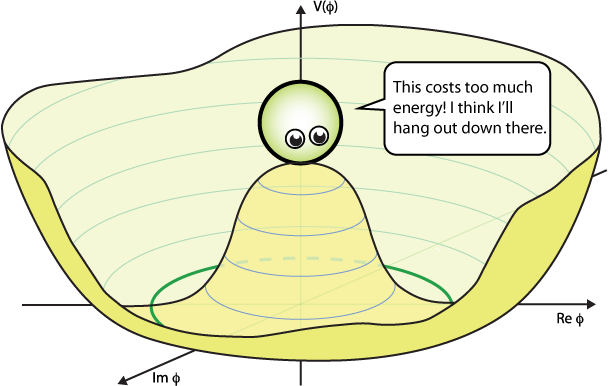
\includegraphics[width = .45\textwidth]{higgs_field.png}
    \caption{Visualization of the Higgs fields, when losing energy. After excitation, it falls down a random direction in the complex plane of the field. All directions have the same magnitude.}
    \label{fig: higgs_field}
\end{figure}

\subsubsection{Higgs Boson Decays}
\begin{itemize}
  \item Does not couple to color charges
  \item Can decay into a the top quark when its a virtual particle, with mass equal to the Higgs boson. Creating an top-antitop pair preserves color charge. This can also produce gluons. 
  \item While photons do not have mass, they can create leptons which later decay into photons.
  \item Some decay channels lead to four leptons. These are easy to detect and were seen as the golden path to finding the Higgs boson. The channel is very rare. 
  \item Some valid vertices are: 
  \begin{itemize}
    \item First order:
    \begin{align}
      &H → W^{+} W^{-} \\
      &H → Z^{0} Z^{0} \\
      &H → HH
    \end{align}
    \item Second order:
    \begin{align}
      &HH → W^{+} W^{-} \\
      &HH → Z^{0} Z^{0} \\
      &HH → HH
    \end{align}
  \end{itemize}
\end{itemize}

\subsubsection{Higgs Boson Experiment Summary}
\begin{itemize}
  \item The Higgs boson does not explain anything new, like dark matter etc. As dark matter have mass, the Higgs should help us understand it. 
  \item We have observe all proton-proton collisions. 
  \item We know it couples to vector bosons and 3rd generation fermions. The previous generations are not observed experimentally. 
  \item We have yet to observe the Higgs boson decaying into Higgs bosons.
\end{itemize}